\documentclass[../main/main.tex]{subfiles}
\begin{document}

\section{Arduino IDE}
Opis\cite{elo} .

\section{Szkic programu}

Poniżej zamieszczono schemat funkcji programu.

\begin{figure}[h]
\centering
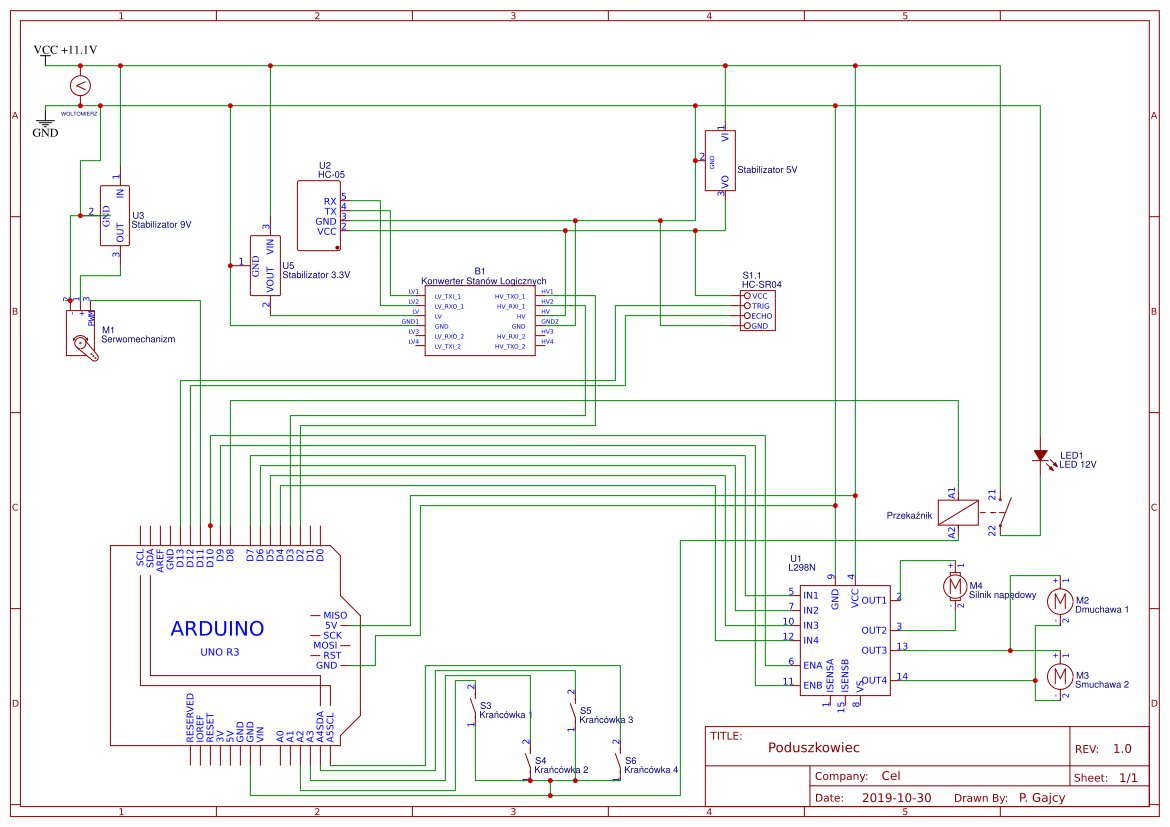
\includegraphics[width=0.75\textwidth]{../obrazy/test.png}
\caption{Wstępny schemat programu sterującego.}
\label{program}
\end{figure}

\section{Funkcje programu}
Spis urządzeń i podzespołów wraz z opisem\cite{shu}.

\subsection{setup}
Setup.

\subsection{loop}
Powtarzanie.

\subsection{Inne funkcje}
L298N

\section{Algorytm działania}
Co ma robić.

\section{Testy}

\end{document}

  
